\documentclass[12pt]{article}
\usepackage{amsmath,amsfonts,amssymb,bbm}
\usepackage{graphicx}

\newenvironment{definition}[1][Definition]{\begin{trivlist}
\item[\hskip \labelsep {\bfseries #1}]}{\end{trivlist}}

\newtheorem{theorem}{Theorem}[section]

\newenvironment{proof}[1][Proof]{\begin{trivlist}
\item[\hskip \labelsep {\bfseries #1}]}{\end{trivlist}}

\begin{document}
\section{Value Remaining}TO DO the naming convention in different. (Utility)\\
Add Matric besides hit rate.
$\mu_{S}=\sum_{x \in S} e^{\beta_{x}}$ is the utility for a given set $S$.\\
Taken ~\cite{scott2015multi} and ~\cite{scott2010modern}, The value remaining in the experiment is the posterior distribution of $\frac{\mu_{max}-\mu_{a^*}}{\mu_{a^*}}$ where $\mu_{max}$ is the largest value of the utility and $\mu_{a^*}$ is the utility of the set that is most likely to be optimal denoted $a^*$. This is constructed as follows, take $n$ Monte Carlo draws from $p(\mu|y_t)$. Let $\mu_{max}^{m}$ be the max utility of draw $m$ and $\mu_{a^*}^{m}$ be the utility using the draw $m$ using the set $a^*$. Let $\Delta^{m}=\frac{\mu^m_{max}-\mu^m_{a^*}}{\mu^m_{a^*}}$.\\
\begin{table}
\begin{center}
\begin{tabular}{l | c c c c c c c c}
Current & 1st &  2nd  &  3rd  &  4th &  5th & 6th & 7th &  8th \\
\hline
Draw 1 & 4.02 &  3.50 &  5.08 & 4.16&  4.22 & 4.41 & 3.65 &  3.27 \\
Draw 2 &4.18 & 4.72 & 3.49 & 3.48 & 3.63 & 3.60 & 3.56 &  3.70 \\
Draw 3 &4.81 & 5.23 & 5.04 &  3.96 &  4.17 & 4.37 &  3.58 & 2.99 \\ 
\end{tabular}
\end{center}
\caption{Draws of utility scores after 100 iterations}
\label{table:data}
\end{table}

\begin{figure}
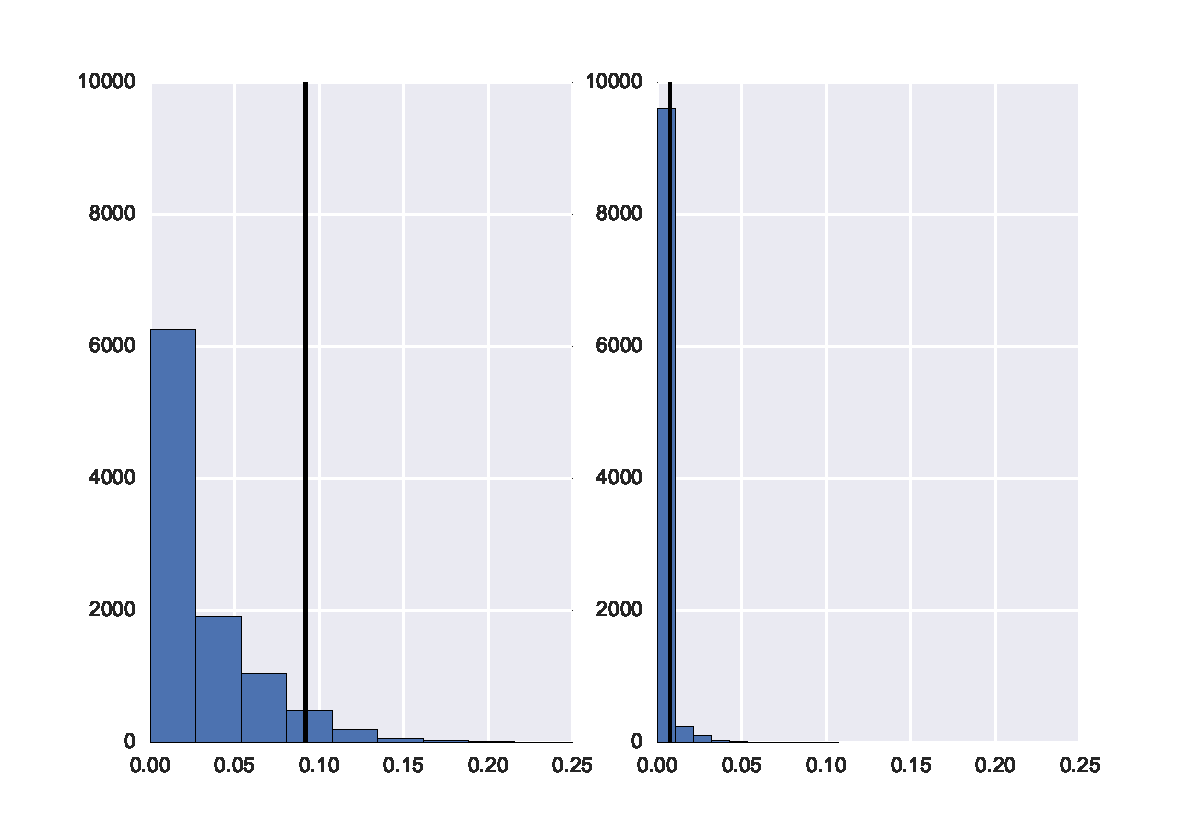
\includegraphics[width=1\linewidth]{valremhist.pdf}
\caption{Two histograms of $\Delta$. Left: After 100 iterations, the potential value remaining is .092. Right: After 220 iterations, the potential value remaining is .008}
\label{fig:data}
\end{figure}

As an example I took draws after respondent 100 in TS $\epsilon=.67$ $\delta=10$ for 120 items see table \ref{table:data} for draws of utility of a single item. I put the columns in current rank order and only show the top 8 for convenience. Say we were finding the value remaining for the the utility score using the top 3. Then $a^*=\{1,2,3\}$. Then $\mu^1_{a^*}=4.02+3.50+5.08=12.6$ and $\mu_{max}^{1}=5.08+4.41+4.16=13.65$ So $\Delta^{1}=\frac{13.65-12.6}{12.6}=.083$. Likewise $\Delta^{2}=\frac{12.6-12.39}{12.39}=.017$ and $\Delta^{3}=\frac{15.08-15.08}{15.08}=0$ (Note $\Delta^m=0$ when the $a^*$ contains the top utilities). The histogram of $\Delta$ after 100 iterations and 220 iterations is shown in figure \ref{fig:data}. \\
 The `potential value remaining' (PVR) is the .95 quantile of the distribution $\Delta$ which in this case was .092. A way to interpret this number is ``We do not know what the utility of $a^*$ is, but whatever it is, a different set might beat it by as much as 9.2\%.''\\
 A good stopping rule is to stop when the PVR drops below a certain threshold, (We use .02 or .05). One advantage of this is it handles ties (two sets with close utility scores) really well. 

\bibliography{source}{}
\bibliographystyle{plain}

\end{document}
